\chapter{Metodologia}\label{meto}


\section{Metodologia Proposta}\label{intro:metodologia}

O objetivo deste projeto é propor um sistema preditivo de Suporte à Decisão que dê apoio a um gestor  quando decidir enviar uma frota de caminhões por determinada rodovia que apresente retenções crescentes 
de logística de cargas.\\

A malha viária está representada na Internet em mapas de bases vetoriais que pretendemos integrar ao nosso sistema de informações e também vamos incorporar as informações que a Polícia Rodoviária Federal(PRF) dispõe, que controla as rodovias BRs. Estas informações estão disponíveis em base de dados históricas nos servidores da PRF além de outras informações para complementar o sistema estão disponíveis na Internet sendo atualizadas pela PRF através de uma API aberta, esta pode ser configurável para se ligar facilmente ao nosso sistema. 

Para representação da malha logística serão utilizadas bases vetoriais, por exemplo, o Google Maps.
Para o desenvolvimento do modelo preditivo pretende-se utilizar bases de dados históricas, por exemplo: da Polícia Rodoviária Federal (PRF), do Centro de Previsões de Tempo e Estudos Climáticos (CPTES - INPE) e possivelmente do Instituto Brasileiro de Geografia e Estatística (IBGE).\\

Para simulação interativa da estrutura preditiva com a dinâmica real serão capturados ``feeds'' de redes sociais, por exemplo pelo Twitter. Essa técnica fará um arco cibernético mantendo o sistema preditivo atualizado.

Propomos um plano que contemple 3 etapas, cada uma dividida em fases atinentes. A figura 3.1 ilustra essa metodologia descrita graficamente, onde as três etapas são representadas por retângulos.
 
\begin{figure}[ht]
\centering
\caption{Etapas da metodologia}
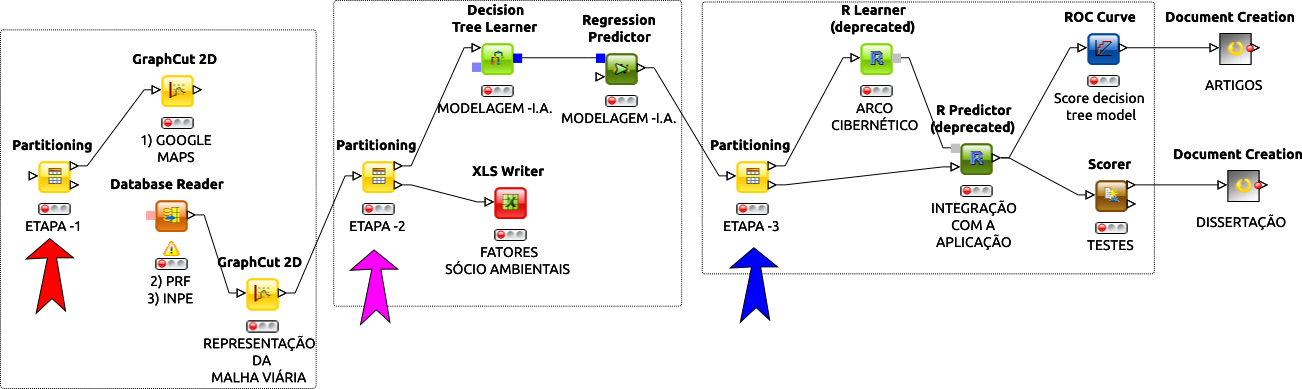
\includegraphics[width=150mm, height=60mm]{Figuras/BigData/Etapas.png}
\end{figure}

 

 \pagebreak
 O retângulo da esquerda é a etapa 1, onde há a representação da malha viária.
 A etapa 1 contempla as fases da coleta das bases vetoriais, das bases de dados históricas e proposição de um modelo de representação único.
 
 O retângulo central é a etapa 2, que consiste nas fases de Identificação dos fatores sócio ambientais na bases históricas, a modelagem do sistema preditivo e aplicação das técnicas de IA. Propomos inicialmente a Regressão Logística e Árvores de decisão, testes iniciais e depuração do modelo.
 
 A última etapa da nossa proposta metodológica é a etapa 3, esta conterá um arco cibernético construído com os dados de redes sociais, como por exemplo a API do Twitter, este ``per si'' fará com que o modelo preditivo seja retro-alimentado, 
 mantendo-o, ao longo do tempo atualizado na perspectiva do usuário gestor. Isso pois, modelos preditivos com o passar do tempo tendem a desfasar-se. Uma proposta algorítmica para substituir a API das redes sociais 
 poderá ser desenvolvida e testada numa fase complementar, o algorítmo Ant-Miner poderá vir a ser um candidato de adaptação.
 
 Concluída as três etapas e com as informações geradas pelo modelo serão escritos artigos científicos  pertinentes à pesquisa em lide e a escrita da dissertação.
 
 
 
 
\section{Cronograma}\label{intro:cronograma}


\begin{table}[htbp]
 \scriptsize
      \centering  \caption{Cronograma -- 12 meses}
	\begin{tabular}{l|c|c|c|c|c|c|c|c|c|c|c|c}
	\hline
	\textbf{Etapas/2016} & \textbf{Fev} & \textbf{Mar} & \textbf{Abr} & \textbf{Mai}& \textbf{Jun} & \textbf{Jul} & \textbf{Ago} & \textbf{Set} & \textbf{Out} & \textbf{Nov} & \textbf{Dez} & \textbf{Jan/17} \\
	  \hline
	  Rev. da literatura. & x & x & x & x & x & x & x & --- & --- & --- & --- & --- \\ \hline
	  Etapa -- 1 & x & x & x & --- & --- & --- & --- & --- & --- & --- & --- & --- \\ \hline
	  Etapa -- 2 & --- & --- & --- & x & x & x & --- & --- & --- & --- & --- & --- \\ \hline
	  Etapa -- 3 & --- & --- & --- & --- & --- & --- & x & x & x & --- & --- & --- \\ \hline
	  Escrita de artigos & --- & --- & --- & --- & --- & --- & --- & --- & x & x & x & --- \\ \hline
	  Escrita da dissertação & --- & --- & --- & --- & --- & --- & --- & --- & x & x & x & --- \\ \hline
	  Defesa & --- & --- & --- & --- & --- & --- & --- & --- & --- & --- & --- & x \\ \hline
	\end{tabular}
\end{table}


 



